\documentclass{beamer}
\usetheme{metropolis}           % Use metropolis theme
\usepackage[outputdir=./.latex-out]{minted} % TODO slet hvis du ikke bruger minted
\newcommand{\tex}[1] {
  \mintinline{latex}{#1}
}
\usepackage{listings}
\title{\LaTeX Webinar}
\date{\today}
\author{Benjamin Rotendahl}
\institute{Study Now}
\begin{document}
\maketitle
\section{Welcome! }
 \begin{frame}{Iteneray }
   The purpose of this webinar is to introduce you to the basics of LaTeX, such
   that you have the necessary knowledge to start writing your own documents.
   This webinar covers:
   \begin{itemize}
     \item Who do you compile \LaTeX and turn source code into a PDF \pause
     \item The syntax and common expressions \pause
     \item Math typesetting \pause
     \item Graphs, tables, and code
   \end{itemize}
 \end{frame}

 \begin{frame}{From code to pdf}
   \LaTeX{} is different from applications such as word, google docs, etc. it's
   not a so called:\emph{WYSIWYG}\footnote{What you see is what you get} editor.
   \pause
   In stead of pressing a button to add emphasis you write:
   \centering\tex{\emph{I'm important}}
 \end{frame}

 \begin{frame}{From code to pdf}
   \begin{figure}[h]
     \centering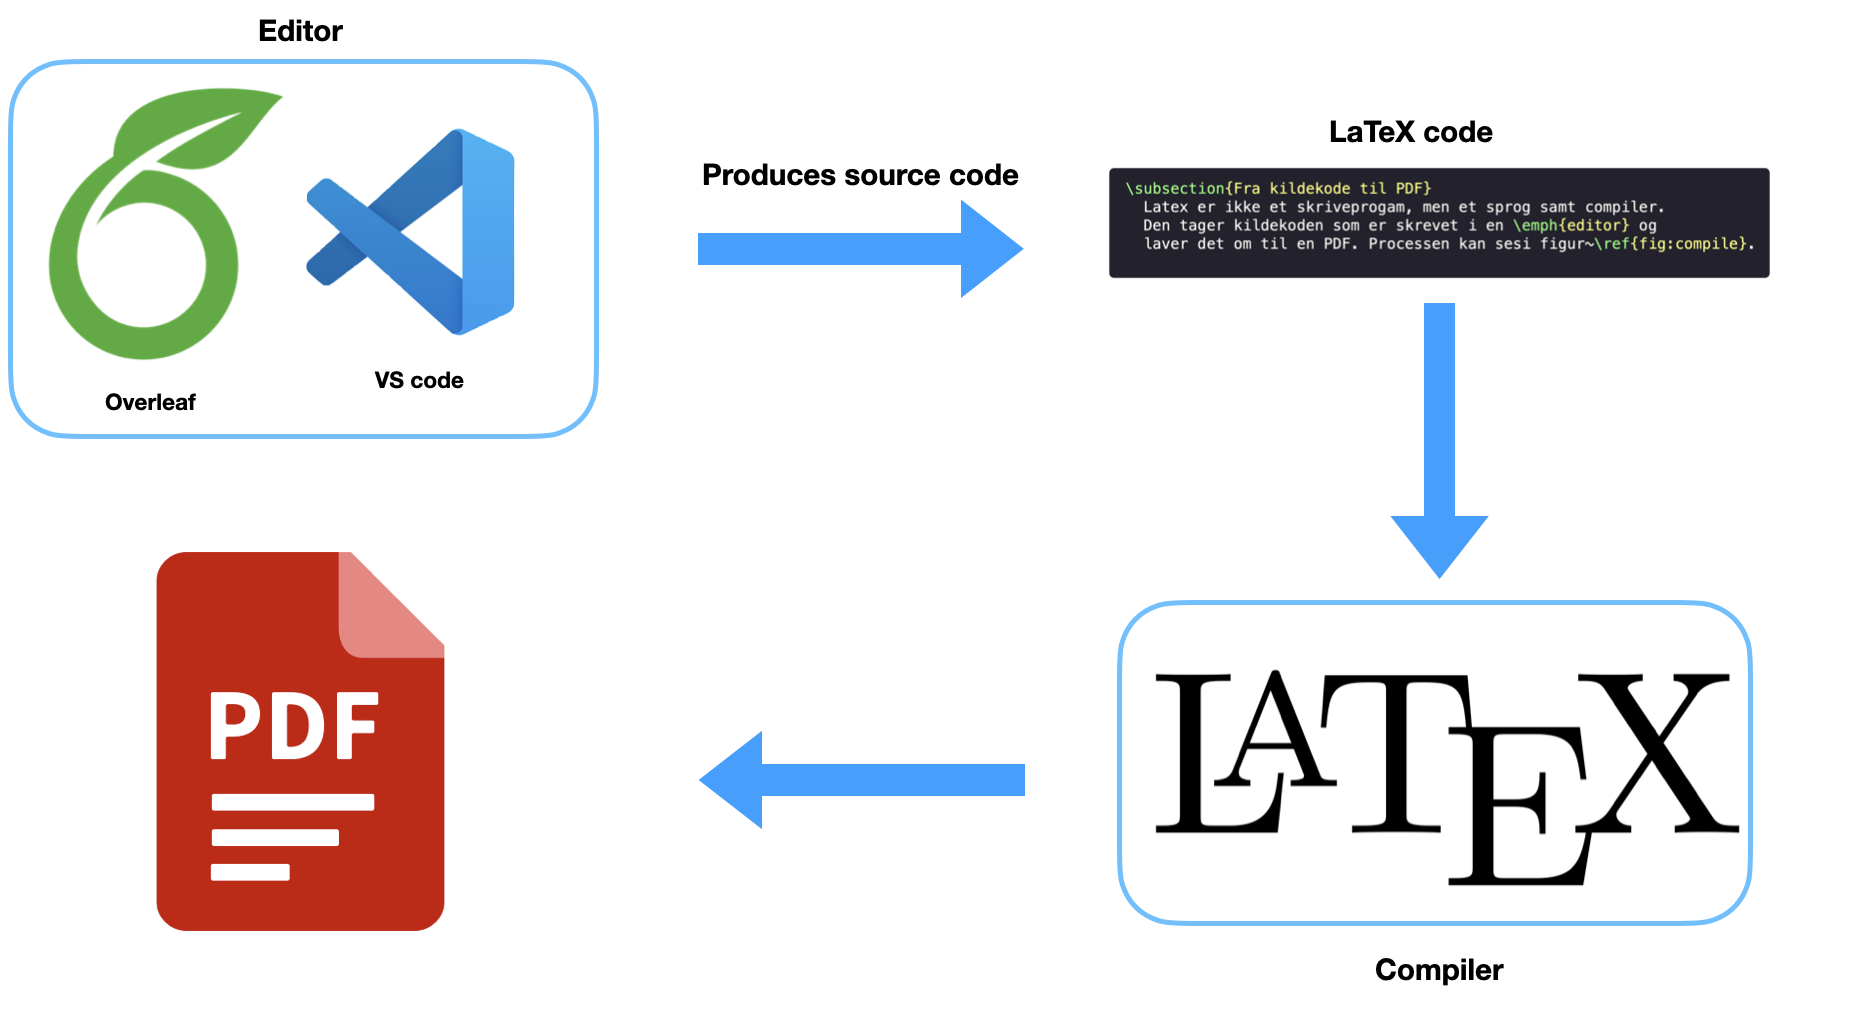
\includegraphics[width=0.9\textwidth]{../assets/compile_en.png}
     \caption{The compilation process}\label{fig:compile}
   \end{figure}
 \end{frame}

 \begin{frame}{\LaTeX styrker}
   The primary strength of \LaTeX is its ability to write mathematical expressions
   \begin{flalign}
     f(x, y)                       & = 3x^2y + y^2 +  \left ( \frac{2^3}{6} \right )^2 \\
     \frac{\partial f}{\partial x} & = 6xy                                             \\
     \frac{\partial f}{\partial y} & = 3x^2 + 2y                                       \\
     \mathbf{z}                    & =  \begin{pmatrix}
                                            1 & 2 & 3 \\
                                            4 & 5 & 6 \\
                                            7 & 8 & 9
                                          \end{pmatrix}
   \end{flalign}
 \end{frame}

\end{document}